\section{Quantisation and Normalization Group Flow}
\label{sec:Renormalization}

This section will treat \emph{scalar perturbative quantum field theory}. We will start by giving a general introduction to the matter and then talk about the \emph{Renormalization group equation}. After introducting \emph{Feynman graphs}, we will finally arrive at the first full definition of a \emph{QFT} and discuss some immediate results. Finally we will discuss the \emph{renormalization of QFT}.

\subsection{Introduction}
\label{subsec:quantisation_intro}

The main idea of Quantum mechanics is to define a deterministic evolution of a system as a superposition of possible evolutions where one weights them by how likely they are. Our ultimate goal is to describe Quantum mechanics and Classical mechanics in terms of the sets of objects, states and observables. The main idea is to take a state $\omega$ and an observable $A$ such that the state associates a propability distribution to the observable on the real line in the form of $\omega_A(\lambda)$. To illuminate the concepts and systems we aim to unify, we present a short overview of both:\\

In Classical mechanics, states are nothing but normalized measures on the \emph{phase space} (mind: a symplectic manifold). Meanwhile observables are functions on the phase space given by $(p,q)$ such that $\omega = dp \wedge dq$. The propability distribution is then given by
$$ \omega_A (\lambda) := \int_M \theta(\lambda - f_A (p,q)) d \mu_\omega$$
where $\theta$ denotes the step function, $f_A$ an observable and $d\mu_\omega$ a measure corresponding to the state. The dynamics on the other hand are encoded in the \emph{Poisson brackets} defined using the symplectic form $\omega$ as
$$ \dd{f}{t} = \{H, f\} $$
for some functions $H$ which turns out to be the \emph{Hamiltonian} of the system.\\

In Quantum mechanics, observables are linear operators on some complex \emph{Hilbert spae} $\HH$. States are positive trace-class operators with unit trace defined as $\Tr A = \sum_n \langle A e_n, e_n \rangle$. The propability distribution for a state is defined by
$$ \omega_A (\lambda) := \Tr(M P_A(\lambda)) $$
where $M$ is a trace-class (state) and $P_A(\lambda)$ is a projection (observable). Note that we are looking at the field from a mathematical perspective, thus the reader might encounter unfamiliar technical details in this and upcoming discussions.\\
The commutator of two states $A,B$ is defined as
$$ \{A,B\} = \frac{i}{\hbar} (AB-BA) $$
such that the time evolution, given the Hamiltonian operator $H$, is defined as
$$ \dd{A}{t} = \{H,A\} $$
With these classifications of the two fields in mind, we arrive at a first sketch of a transition between them:

\begin{definition}[Quantisation Scheme]
  A map passing from Classical mechanics to Quantum mechanics is called a \textbf{quantisation scheme}.
\end{definition}

To illuminate this rather vague definition, we discuss a "toy example":

\begin{example}[Weyl Quantisation]
  This quantisation treats a mechanical system with one degree of freedom. The classical system has $\RR^2$ as its phase space with coordinates $(p,q)$. The dynamics are given by the Poisson-brackets with the Hamiltonian function. Now we want to transition to a quantum description:\\

  We take the Hilbert-space $\HH$ defined as
  $$ \HH = L^2(\RR) := \{ \psi(q) \in C(\RR) \ | \ \int_{-\infty}^\infty |\psi(q)|^2 dq < \infty  \} $$
  Observables are now operators on $\HH$. We define the two operators
  $$ (P\psi)(q) = \frac{\hbar}{i} \dd{}{q} \psi(q), \quad \quad (Q\psi)(q) = q \psi(q) $$
  Now we can define products
  $$ (A\psi)(q) = \int_{-\infty}^\infty A(q,q^\prime) \psi(q^\prime) dq^\prime $$
  where $A(q,q^\prime)$ denotes the integral kernel of $A$ defined as
  $$ A(q,q^\prime) = \frac{1}{2 \pi \hbar} \int_{-\infty}^\infty f\left( p, \frac{q+q^\prime}{2} \right) e^{ip(q-q^\prime)/\hbar} dq $$
  where the $f$ are functions that represent $A$ in classical mechanics. As an exercise you can show that with these definitions you obtain the previously defined operators $P,Q$ if you set $f=p$ and $f=q$ respectively.\\

  Next we need to define a product. Since generally $A_{fg} \neq A_f A_g$ we investigate
  $$ A_f A_g (q, q^\prime) = \int_{-\infty}^\infty A_f(q, q^{\prime \prime}) A_f(q^{\prime \prime},q^\prime) dq^{\prime \prime} $$
  and then define
  $$ f *_\hbar g = fg + \frac{i\hbar}{2} \{f,g\} + \mathcal{O}(\hbar^2) \quad \Rightarrow \quad \frac{i}{\hbar} (f *_\hbar g - g *_\hbar f) = \{f,g\} + \mathcal{O}(\hbar^2)$$
  We now encode the dynamics via the time derivative using the Hamiltonian operator
  $$ \dd{A(t)}{t} = \{H, A(t)\}_\hbar , \quad \quad A(0) = A $$
  where we define $A(t)$ as
  $$ A(t) = U^{-1}(t) A U(t), \quad \quad U(t) = e^{-i H t / \hbar} $$
  As an exercise you can prove this in a formal setting. Note that we do not yet have a concrete way to define the exponential of an operator such as $H$. Thus, setting $\hbar = 1$ for simplicity, we investigate the integral kernel of $U = e^{-iH(t^{\prime \prime} - t^\prime)}$ in terms of $h(p,q)$. To this end let $\Delta << 1$ such that
  $$ U_\Delta := e^{-i H \Delta} \cong 1- i H \Delta $$
  Thus setting $t^{\prime \prime} - t^\prime = N \Delta$ we obtain $e^{-iH(t^{\prime \prime} - t^\prime)} = (U_\Delta)^N$. Now we calculate
  \begin{align*}
    U_\Delta(q,q^\prime) &= \frac{1}{2\pi} \int_{-\infty}^\infty dp e^{ip(q-q^\prime)} \left( 1- i h\left(p, \frac{q+q^\prime}{2} \right) \Delta \right) \\
    &= \frac{1}{2\pi} \int_{-\infty}^\infty dp e^{ip(q-q^\prime) - i h\left(p, \frac{q+q^\prime}{2} \right) \Delta} + \mathcal{O}(\Delta^2)
  \end{align*}
  Now setting $q = q_N, q^\prime = q_0$ and $q_j$ the $N-1$ intermediate variables, we arrive at the following form:
  \begin{align*}
    U(q, q^\prime, t^{\prime\prime}-t^\prime) &= \int_{-\infty}^\infty ... \int_{-\infty}^\infty \frac{dp_1 dq_1}{2\pi} ... \frac{dp_{N-1} dq_{N-1}}{2\pi} \frac{dp_N}{2\pi}\\
    &\times e^{ip_{N}(q_{N}-q_{N-1}) + ... + ip_1(q_1-q_0)} \cdot e^{-ih\left(p_N, \frac{q_N + q_{N+1}}{2}\right) ... -ih\left( p_1, \frac{q_1 + q_0}{2} \right)}
  \end{align*}

  Thus we take $N\lra \infty$ such that $q_j - q_{j-1}$ being proportional to $\frac{1}{N}$ goes against $0$. While we do not discuss convergence and well-definedness at this point, the reader is invited to start looking critically at these notions from now on! Formally this gives us the following form of $U$ which indeed has many problems with convergence of integrals
  \begin{align*}
    U(q,q^\prime, t^{\prime\prime}-t^\prime) = \int ... \int_{t^\prime}^{t^{\prime\prime}} \prod_i \frac{dp(t) dq(t)}{2\pi} \exp\Big[dt i ( p(t)\dot q(t) - h(p(t),q(t)))\Big]
  \end{align*}
  Where the first fraction defines our measure on the space of paths from $[t^\prime, t^{\prime\prime}]$ called the \textbf{Liouville-measure} and the term in the exponential is called the \textbf{Action functional}.\\

  Note that this is only a one-dimensional "toy model" which already boasts some pretty severe convergence problems. Since we ultimately aim to define an infinite-dimensional generalization, the rest of the course will deal with the "taming" of these problems.
\end{example}

In the following we give a short introduction to \textbf{Feynman Path Integrals}, visually respresented in the following picture:
\begin{center}
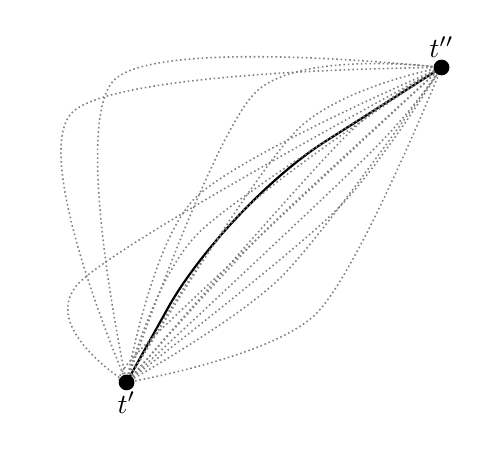
\begin{tikzpicture}[]
\draw[thick, black,rounded corners=15mm] (-2.,-2.) -- (-.75,.25) -- (2,2);

\foreach \j in {1,...,15} {
  \draw[gray,densely dotted, line width = .2mm] plot[smooth] coordinates {(-2.,-2.)(-.75+2*rand,.25+2*rand)(2,2)};
}

\fill [black] (2.,2.) circle (0.1) node[above]{$t^{\prime\prime}$};
\fill [black] (-2.,-2.) circle (0.1) node[below]{$t^\prime$};
\end{tikzpicture}
\end{center}
Feynman's approach to Quantum Field Theory was the idea of a "sum over all possible histories" of a particle. In \emph{chapter 2} \ref{subsec:Classical_field_theory} we already mentioned scalar field theories where $\psi \in\Ci(M)$ is a scalar field. The physical phenomenon corresponding to the "sum over histories" is described by a superposition of all possible scalar theories, weighted by $e^{iS(\psi) / \hbar}$ for $S(\psi)$ the action of $\psi$.\\

This in turn has an interpretation coming from statistical mechanics: Here, $\psi$ would represent the state of a statistical system, $S(\psi)$ would be the systems energy. Given a temperature $T$, the system could be in any state $e^{-S(\psi)/ T}$. Thus we obtain the following correspondence:
\begin{center}
\begin{tikzcd}
  T \arrow[r,leftrightarrow] & i \hbar
\end{tikzcd}
\end{center}
This gives us a sufficient motivation to repeat the assessment of dynamics for statistical systems:\\

In statistical mechanics, observables are maps $O: \Ci(M,\RR) \lra \CC$ and correlation functions between observables are defined as
\begin{align*}
  \langle O_1, ..., O_n \rangle &= \int_\psi e^{-S(\psi)/T} O_1(\psi) ... O_n(\psi) D\psi\\
  \Longrightarrow \quad \quad \langle O_1, ..., O_n \rangle &= \int_{\psi \in \Ci(M)} e^{i S(\psi)/\hbar} O_1(\psi) ... O_n(\psi) D\psi
\end{align*}
The main problem in this situation is that $\Ci(M)$ is an infinite-dimensional vector space.

\begin{rem}~
\begin{itemize}
  \item[(1)] One approach to resolve this is \emph{perturbative QFT} where we work in the limit $\hbar \lra 0$ such that we can take formal power series in $\hbar$. This provides us with a formal procedure to go from a quantum description to a classical one. Note that this endows $\hbar$ with the role of a formal parameter.

  \item[(2)] In addition to a perturbative treatment, we can drop the Lorentzian signature and stick to Riemannian ones since the mathematical background is better understood.
\end{itemize}
\end{rem}


\subsection{The Effective Action}
\label{subsec:effective_action}

In this section, we try to "tame" the previously exposed integrals over infinite-dimensional vector spaces. We were stuck with expressions of the form $\langle O_1, ..., O_n \rangle$ which indeed could not be calculated with the tools we previously used. One approach to expressions of this form are \emph{"Wilson low-energy theories"} which will make up the first part of this subchapter.\\

The main idea of \emph{"Wilson low-energy theories"} is that observables can only measure phenomena with an energy below a fixed constant energy $\Lambda$. Thus let us fix a Riemannian manifold $M$, $I \subset [0,\infty)$ and denote by $\Ci(M)_I \subset \Ci(M)$ the set of functions $f$ that are sums of eigenfunctions of the \emph{Laplacian} \ref{def:codifferential} with eigenvalues in $I$.

\begin{lem}
  If $I$ is bounded, $\Ci(M)_I$ is a finite-dimensional vector space.
\begin{proof}
  The proof is left as an exercise to the reader.
\end{proof}
\end{lem}

Now let $\Lambda \in I$ and define $J = [0,\Lambda)$. We thus define
$$ \Ci(M)_J := \Ci(M)_{\leq \Lambda} \subseteq \Ci(M) $$
and call it the \textbf{space of fields with energy at most $\Lambda$}. Observables in this framework, i.e. restricted to such fields, are functionals
$$ O \colon \Ci(M)_{\leq \Lambda} \lra \RR\llbracket\hbar\rrbracket $$
where $\RR\llbracket\hbar\rrbracket$ denotes formal power series in $\hbar$. We can extend each such operator $O$ to $\Ci(M)$ by composing it with the evident projection to $\Ci(M)_{\leq \Lambda}$. We define $Obs_{\leq \Lambda}$ to be the thus arising observables.\\

Now we investigate $\langle O_1, ..., O_n \rangle$ where $O_i \in Obs_{\leq \Lambda}$. We define quantities of this form as
$$ \langle O_1, ..., O_n \rangle := \int_{\phi \in \Ci(M)_{\leq \Lambda}} e^{S_{eff}[\Lambda](\phi) / \hbar} \ O_1 ... O_n \ D\phi$$
Here, $D\phi$ is the Lebesgue measure on $\Ci(M)_{\leq \Lambda}$, $S_{eff}[\Lambda]$ is a function on $\Ci(M)_{\leq \Lambda}$ and thus a formal power series in $\hbar$. We call such an action a \textbf{low energy effective action}.

\begin{rem}
  The quadratic part of $S_{eff}[\Lambda]$ is negative-definite.
\end{rem}

\begin{definition}(Scalar Quantum Field Theory)
\label{def:scalar_qft}
  A \textbf{scalar (perturbative) quantum field theory} is a collection of effective actions
  $$ S_{eff}[\Lambda]\colon \Ci(M)_{\leq \Lambda} \lra \RR\llbracket\hbar\rrbracket $$
  for all $\Lambda \in [0,\infty)$ such that
  \begin{enumerate}
    \item $S_{eff}[\Lambda]$ is a formal power series in both the field $\phi \in \Ci(M)_{\leq \Lambda}$ and the variable $\hbar$.

    \item Modulo $\hbar$, $S_{eff}[\Lambda]$ must be of the form
    $$ S_{eff}[\Lambda] = - \frac{1}{2} \int \phi (D + m^2) \phi + \mathcal{O}(\phi^3) $$
    where $D$ is the positive-definite Laplacian.

    \item If $\Lambda^\prime \leq \Lambda$, $S_{eff}[\Lambda^\prime]$ is determined by $S_{eff}[\Lambda]$ by the renormalisation group equation.

    \item The effective actions $S_{eff}[\Lambda]$, when translative in length scale terms, satisfy the asymptotic locality axiom.
  \end{enumerate}
  \emph{Note that the notions mentioned in points 3. and 4. have not been discussed yet. To fill in these gaps will be the function of this subchapter.}
\end{definition}

We will subsequently fix the notions mentioned in the previous definition. From point $2.$ we know that $S_{eff}[\Lambda]$ must be of the following form:
$$S_{eff}[\Lambda](\phi) = - \frac{1}{2} \langle \phi, (D+m^2)\phi \rangle + I[\Lambda](\phi) $$
Here, $\langle \cdot , \cdot \rangle$ denotes the $L^2$-inner product on $\Ci(M)$ defined via
$$ \langle \phi , \psi \rangle := \int_M \phi(x) \psi(x) dx$$
$D$ is the Laplacian and $m$ is a positive real parameter. Further, $I[\Lambda]$, the \textbf{effective interaction}, is understood as a formal power series in $\hbar$:
$$ I[\Lambda](\phi) = I_0[\Lambda](\phi) + \hbar I_1[\Lambda](\phi) + ... $$
Here, $I_0[\Lambda](\phi)$ is at least cubic in $\phi$ and all the $I_i$ are formal power series in $\phi$.\\

\subsection{Renormalization group equation}
\label{subsec:renorm_group_eq}

Now our goal is to "translate" a system $S_{eff}[\Lambda], Obs_{\leq \Lambda}, \Ci(M)_{\leq \Lambda}$ into one with threshold $\Lambda^\prime \leq \Lambda$. There exists an evident inclusion $Obs_{\leq \Lambda^\prime} \hookrightarrow Obs_{\leq \Lambda}$. The correlation functions should not change if we compute them in $Obs_{\leq \Lambda^\prime}$ rather than in $Obs_{\leq \Lambda}$:

\begin{align}
\label{eq:connection_eq}
  \int_{\phi \in \Ci(M)_{\leq \Lambda^\prime}} e^{S_{eff}[\Lambda^\prime] (\phi) / \hbar} \ O_1(\phi) ... O_n(\phi) \ D\phi^{\Lambda^\prime} = \int_{\phi \in \Ci(M)_{\leq \Lambda}} e^{S_{eff}[\Lambda] (\phi) / \hbar} \ O_1(\phi) ... O_n(\phi) \ D\phi^{\Lambda}
\end{align}

Further note that we can split
$$ \Ci(M)_{\leq \Lambda} = \Ci(M)_{\leq \Lambda^\prime} \oplus \Ci(M)_{(\Lambda^\prime,\Lambda]} $$
Using this splitting to separate \eqref{eq:connection_eq} allows us to formulate:

\begin{align*}
  RHS &= \int_{\phi_L \in \Ci(M)_{\leq \Lambda^\prime}}
  \int_{\phi_H \in \Ci(M)_{(\Lambda^\prime,\Lambda]}}
  e^{S_{eff}[\Lambda] (\phi_L + \phi_H) / \hbar} \ O_1(\phi_L) ... O_n(\phi_L) \ D\phi^{\Lambda^\prime} \ D\phi^{\Lambda \Lambda^\prime} \\
  &= \int_{\phi_L \in \Ci(M)_{\leq \Lambda^\prime}}
  \left [\int_{\phi_H \in \Ci(M)_{(\Lambda^\prime,\Lambda]}}
  e^{S_{eff}[\Lambda] (\phi_L + \phi_H) / \hbar} \ D\phi^{\Lambda \Lambda^\prime} \right] \ O_1(\phi_L) ... O_n(\phi_L) \ D\phi^{\Lambda^\prime} \\
\end{align*}
This in turn allows us to identify
$$ e^{S_{eff}[\Lambda^\prime](\phi_L)/\hbar}
= \int_{\phi_H \in \Ci(M)_{(\Lambda^\prime,\Lambda]}}
e^{S_{eff}[\Lambda] (\phi_L + \phi_H) / \hbar} \ D\phi^{\Lambda \Lambda^\prime} $$
which ultimately leads to the \textbf{Renormalisation group equation (RGE)}
\begin{align}
\label{eq:RGE}
  S_{eff}[\Lambda^\prime](\phi_L)
  = \hbar \log \left[ \int_{\phi_H \in \Ci(M)_{(\Lambda^\prime,\Lambda]}}
  e^{S_{eff}[\Lambda] (\phi_L + \phi_H) / \hbar} \ D\phi^{\Lambda \Lambda^\prime} \right]
\end{align}

Having a rather well-defined system of such effective actions we may wonder, what their relation to the original classical action $S$ is. This correspond to a "limit" of the form $S_{eff}[\infty]$ that is $\Lambda \lra \infty$. Note that the space of fields we used in the integral of \eqref{eq:RGE} is ill-defined for $\Lambda = \infty$, thus this discussion is not trivially dispatched.\\

One approach is to describe $RGE$ \eqref{eq:RGE} in terms of effective interactions. Note that $\Ci(M)_{\Lambda^\prime}$ and $\Ci(M)_{\Lambda}$ are $D$-orthogonal, thus
\begin{align*}
  \langle \phi_L + \phi_H , D(\phi_L + \phi_H) \rangle &= \langle \phi_L , D\phi_L \rangle + \langle \phi_H , D\phi_H \rangle \\
  \langle \phi_L + \phi_H , m^2(\phi_L + \phi_H) \rangle &= \langle \phi_L, m^2 \phi_L \rangle + \langle \phi_H, m^2 \phi_H \rangle
\end{align*}

Now if we define
$$ F(\phi) = - \frac{1}{2} \pair{\phi}{(D+m^2)\phi}, \quad \quad s.t. \quad \quad F(\phi_L + \phi_H) = F(\phi_L) + F(\phi_H) $$
we can rewrite our effective action as
$$ S_{eff}[\Lambda](\phi) = F(\phi) + I[\Lambda](\phi), \quad \quad s.t. \quad \quad S_{eff}[\Lambda](\phi_L + \phi_H) = F(\phi_L) + F(\phi_H) + I[\Lambda](\phi_L + \phi_H)$$
Combining this with \eqref{eq:RGE} brings us to
\begin{align*}
  F(\phi_L) + I[\Lambda^\prime](\phi_L) &= \hbar \log \left[  \int_{\phi_H \in \Ci(M)_{(\Lambda^\prime,\Lambda]}} \exp\left(\frac{F(\phi_H)}{\hbar} + \frac{F(\phi_L)}{\hbar} + \frac{I[\Lambda](\phi_H + \phi_L)}{\hbar} \right) \ D\phi^{\Lambda^\prime \Lambda} \right] \\
  &= \hbar \log \left[ e^{\frac{F(\phi_L)}{\hbar}} \int_{\phi_H \in \Ci(M)_{(\Lambda^\prime,\Lambda]}} \exp\left(\frac{F(\phi_H)}{\hbar} + \frac{I[\Lambda](\phi_H + \phi_L)}{\hbar} \right) \ D\phi^{\Lambda^\prime \Lambda} \right] \\
  &= F(\phi_L) + \hbar \log \left[ \int_{\phi_H \in \Ci(M)_{(\Lambda^\prime,\Lambda]}} \exp\left(\frac{F(\phi_H)}{\hbar} + \frac{I[\Lambda](\phi_H + \phi_L)}{\hbar} \right) \ D\phi^{\Lambda^\prime \Lambda} \right]
\end{align*}

Thus we arrive at the \textbf{Interaction form of the RGE}:
\begin{align}
\label{eq:RGE_interaction}
  I[\Lambda^\prime](\phi_L) = \hbar \log \left[  \int_{\phi_H \in \Ci(M)_{(\Lambda^\prime,\Lambda]}} \exp\left(\frac{F(\phi_H)}{\hbar} + \frac{I[\Lambda](\phi_H + \phi_L)}{\hbar} \right) \ D\phi^{\Lambda^\prime \Lambda} \right]
\end{align}
This form has two major advantages over \eqref{eq:RGE}:
\begin{enumerate}
  \item We are not integrating over $\phi \in \Ci(M)_{\leq \Lambda^\prime}$, the equation can be extended to any $\phi_L \in \Ci(M)$.

  \item It is invertible by choosing $\Lambda^\prime > \Lambda$.
\end{enumerate}

While we have indeed explored the meaning and framework of \emph{point 3.} of \ref{def:scalar_qft}, we still have to settle the notion of \textbf{locality}. On a physical level, locality means that interactions between fundamental particles occur at a point of the manifold.

\begin{definition}[Local action functional]
  A functional $S\colon \Ci(M) \lra \RR \llbracket \hbar \rrbracket$ is a \textbf{local action functional} if it can be written as a sum
  $$ S(\phi) = \sum_k S_k (\phi), \quad \text{where} \quad S_k(\phi) = \int_M (D_1 \phi) ... (D_k \phi) \ \vol_M \ ( \llbracket \hbar \rrbracket)$$
  for some differential operators $D_i$ on $M$. This allows us to write $S$ as
  $$ S(\phi) = \int_M \mathcal{L}(\phi)(x) \ dx $$
  where $\mathcal{L}(\phi)$ is a \textbf{Lagrangian} and depends only on the expansion of $\phi$ at $x$.
\end{definition}




\newpage
